
\section{Simulation}\label{sec:simulation}
This section examines three challenges for torque control of an object, arranged in increasing difficulty.  Each task uses a PD controller that regulates the swarm's mean position,  as in \cite{ShahrokhiIROS2015}. The control input is the global force applied to each robot:
\begin{align}
u_x &= K_{p}(goal_x - \bar{x}) + K_{d}(0-\bar{v}_x) \nonumber\\
u_y &= K_{p}(goal_y  - \bar{y}) + K_{d}(0-\bar{v}_y)  \label{eq:PDcontrolPosition}
\end{align}
here $K_{p}$ is the proportional gain, and $K_{d}$ is the derivative gain.  
The swarm's average position is $[\bar{x},\bar{y}]^T$ and mean velocity is $[\bar{v}_x,\bar{v}_y]^T$.  
Each task uses a different algorithm to select the swarm's goal position $[goal_x,goal_y]^T$. The derivative gain $K_d$ limits overshoot.

\paragraph{Maximizing torque on a pivoted body} \label{sec:simulationPureTorque}
An object with a pivot point can rotate, but not translate. A door is an example.
 If there was only one robot touching the object, the robot should push at the point which maximizes the moment arm, at the extreme end of the object furthest from the pivot point.
% \begin{align}
%\tau = F \times (P - O )\label{eq:torque}
% = F \cdot (P - O )\label{eq:torque}
%\end{align}
The optimal pushing location provides the maximum force, because it maximizes the distance $r = \norm{P - O}$ in \eqref{eq:torque}.
However, given a swarm of robots, maximizing $r$ is no longer the optimal solution.  
If the mean of the swarm hits the object at the extreme edge, half of the robots will miss the object and  the swarm will be split.
Because few robots remain,  the force is significantly decreased and torque is not maximized.
 In our simulation, the swarm applies torque until the swarm's mean position is beyond the object. Then the swarm will regather in a corner before returning to torque control, a time-consuming task. 
 The key parameter of interest for a hinged door of length $L$ is $C$, the position along the door where the mean of the swarm will push.  The goal position in ~\eqref{eq:TorqueControl} is set to:
 
\begin{align}\nonumber
goal_x &= O_x + C \cos(O_{\theta}) \\
goal_y &= O_y + C \sin(O_{\theta}),  \label{eq:TorqueControl}
\end{align}
%\textcolor{red}{??The coordinate frames here are different from the rest of the paper}
$O_{\theta}$ = the orientation of the object's major axis, measured from the world $x$-axis.
 Fig. \ref{fig:LFig} illustrates how different values of $C$ result in different rates of turning. These simulations tested $C = \{1/2, 3/4, 5/8, 1\}L$. The fastest turning rates occurred with  $C =  5/8L$. Code is available at \cite{Shahrokhi16torque}.

%\textcolor{red}{??TODO: PUT THE NEW REAL SIMULATIONS HERE
%SIm 1: include  push at the optimal location
%}
%
%\begin{figure}
%\begin{center}
%	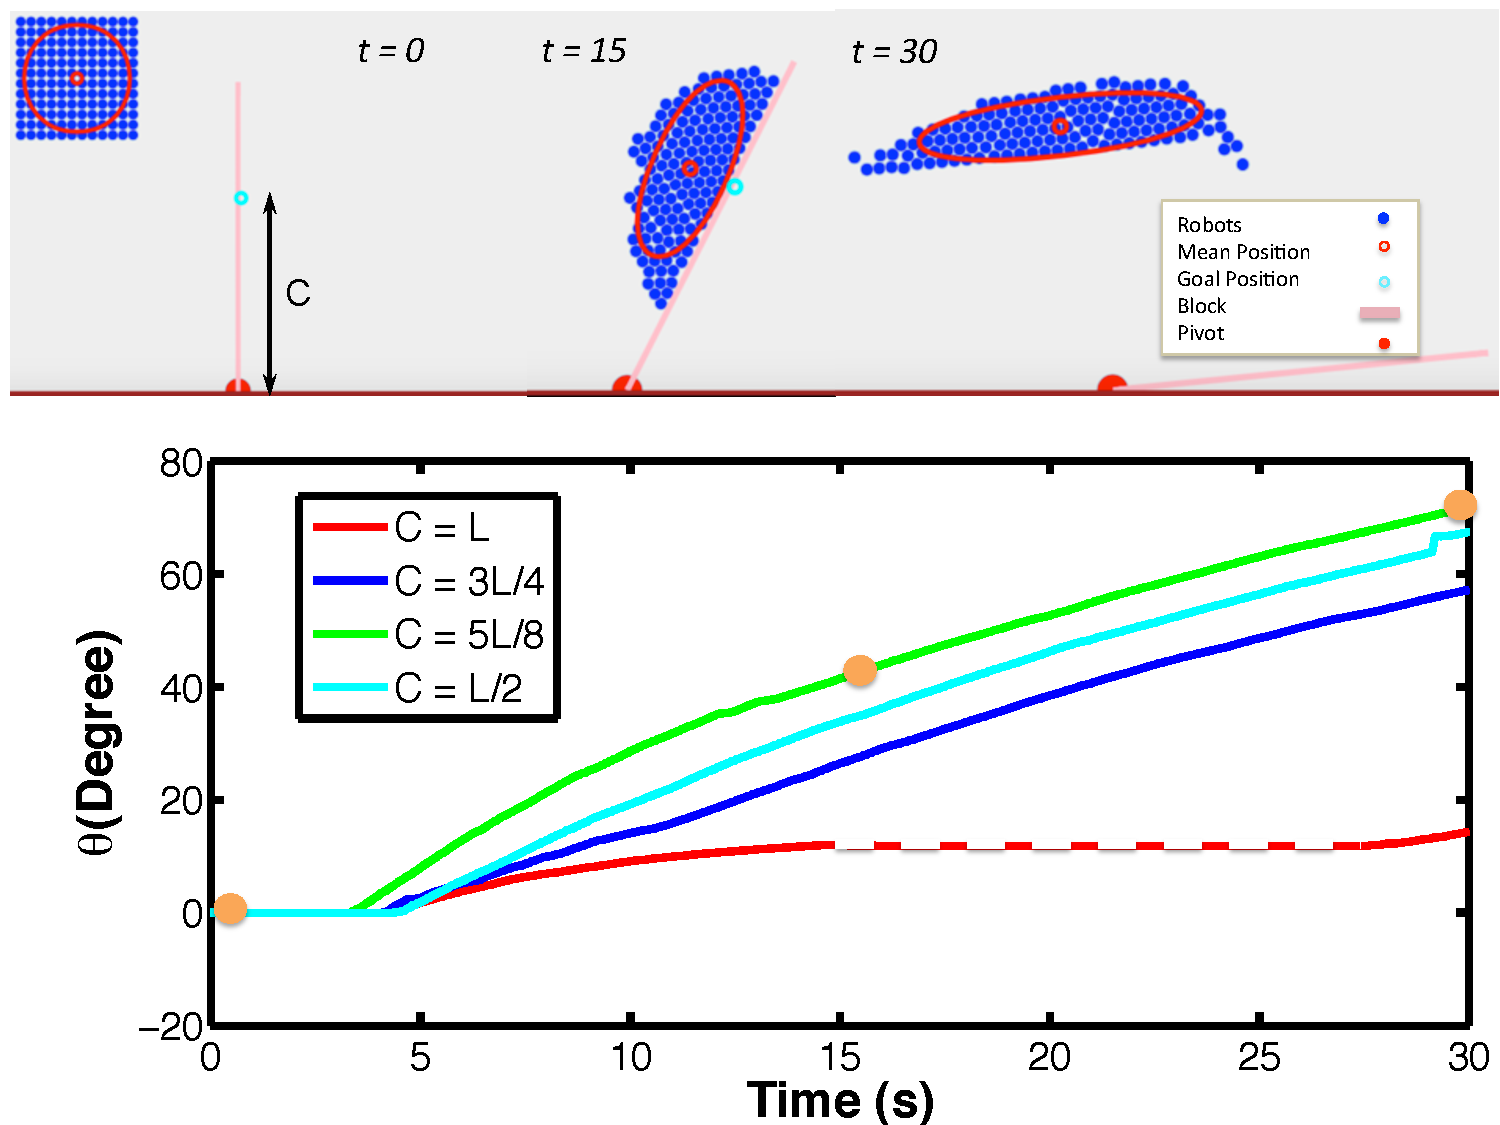
\includegraphics[width=0.8\columnwidth]{LFig.pdf}
%\end{center}
%\vspace{-1em}
%\caption{\label{fig:LFig}
%Simulation results from a swarm applying force to a hinged door. 
%The swarm mean is steered toward a point $C$ units along the object from the pivot point. The red dashed line indicates the times that the swarm was in variance control mode.
% Simulation used 144 robots of diameter $0.2$ m with a standard deviation of less than $1.5$ m and an object length of $6$ m.
%}
%\vspace{-1em}
%\end{figure}


\paragraph{Orientation of the object}
These simulations used a uniform density rectangle as the object. This object was 30$\times$ larger than the robots.
Using the pure torque control discussed in the previous paragraph, the orientation of the object can be controlled by applying force. 
The rectangular object is not pivoted, so it moves in addition to rotating. 
 The swarm still may split into multiple components.
  We use the hysteresis variance control from \cite{ShahrokhiIROS2015}  to gather the swarm when its variance grows too large. 
  The following control law chooses a goal position to regulate the orientation of the object.  
  
 \begin{align}\nonumber
goal_x = O_x +  K_{\textrm{orient}}  (O_{\theta} - goal_\theta ) \cos(O_{\theta}) \\
goal_y = O_y +  K_{\textrm{orient}}   ( O_{\theta} -goal_\theta  ) \sin(O_{\theta})
\end{align}
Here $K_{orient}$ is a positive gain on the control input.  



%\textcolor{red}{??TODO: PUT THE REAL SIMULATIONS HERE.}
%
%\begin{figure}
%\begin{center}
%	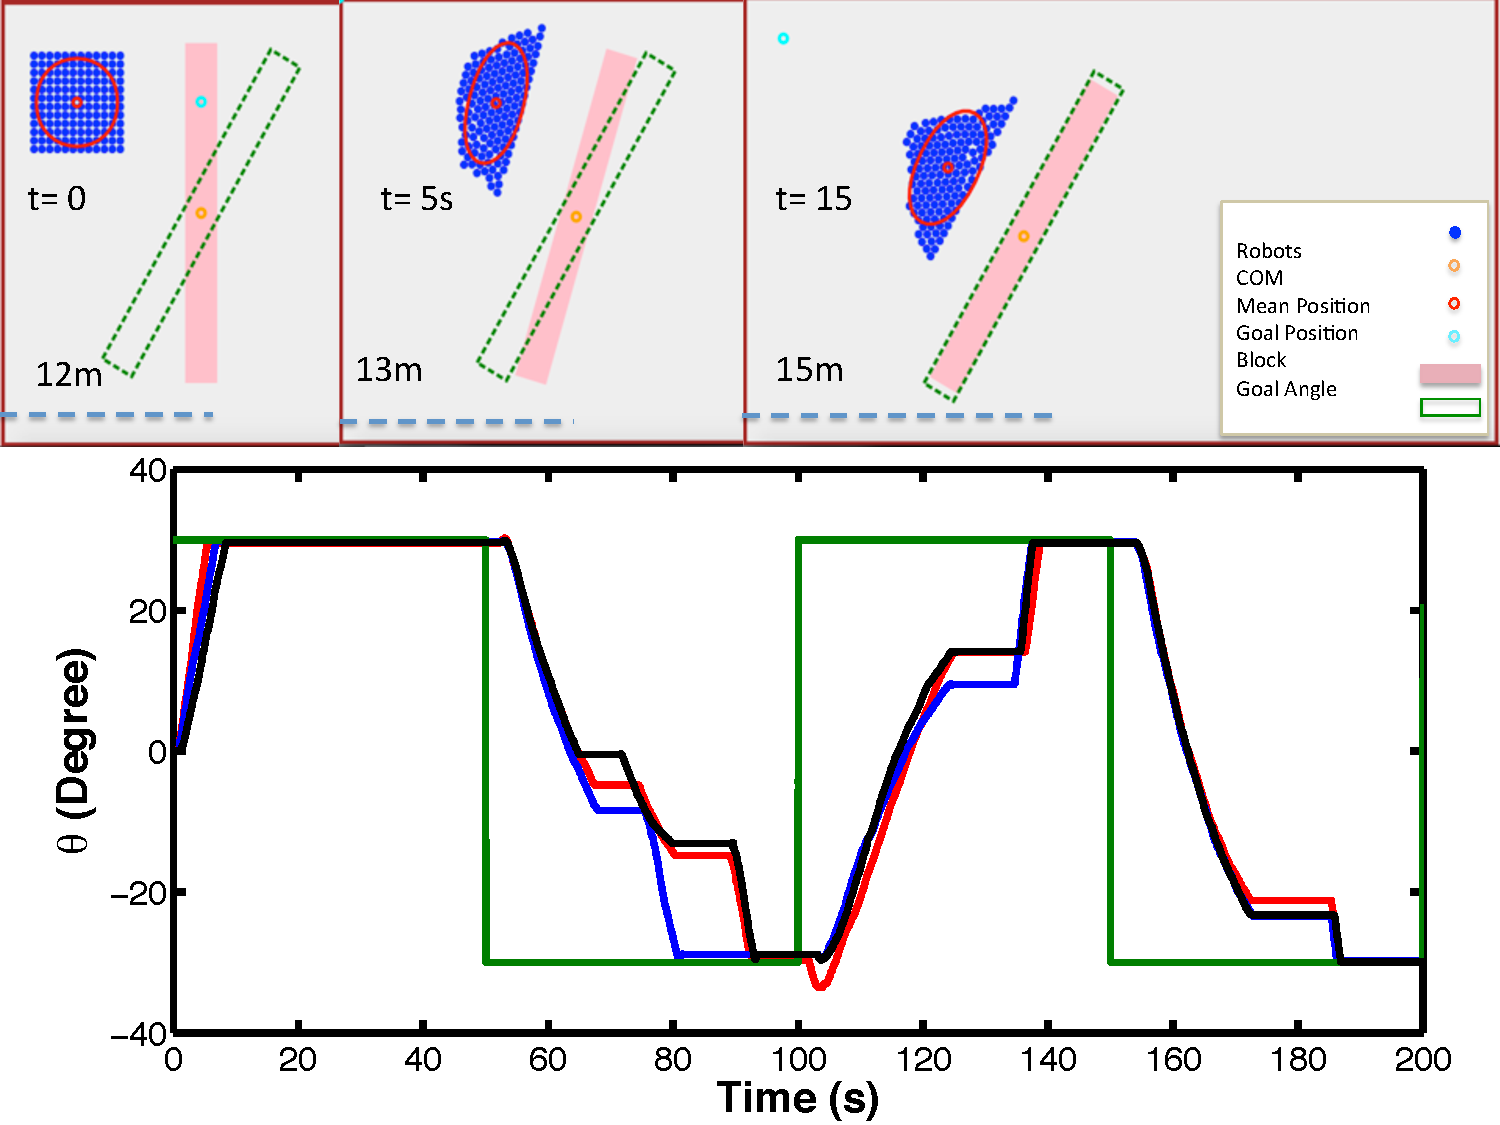
\includegraphics[width=0.8\columnwidth]{Orientation.pdf}
%\end{center}
%\vspace{-1em}
%\caption{\label{fig:OrientCont}
%Plot demonstrating  orientation control of a rectangular object. The green line is the goal orientation. Other lines show different random starting position of the swarm. When the plot traces are constant the swarm is no longer pushing the object and instead is being regathered in a corner of the workspace until the variance is below a desired threshold. 
%}
%\vspace{-1em}
%\end{figure}

Fig. \ref{fig:OrientCont} illustrates this controller with different starting positions. When the plot traces are constant the swarm is no longer pushing the object and instead is being regathered in a corner of the workspace. Code is available at \cite{Shahrokhi16Orient}.




\begin{figure}
\begin{center}
	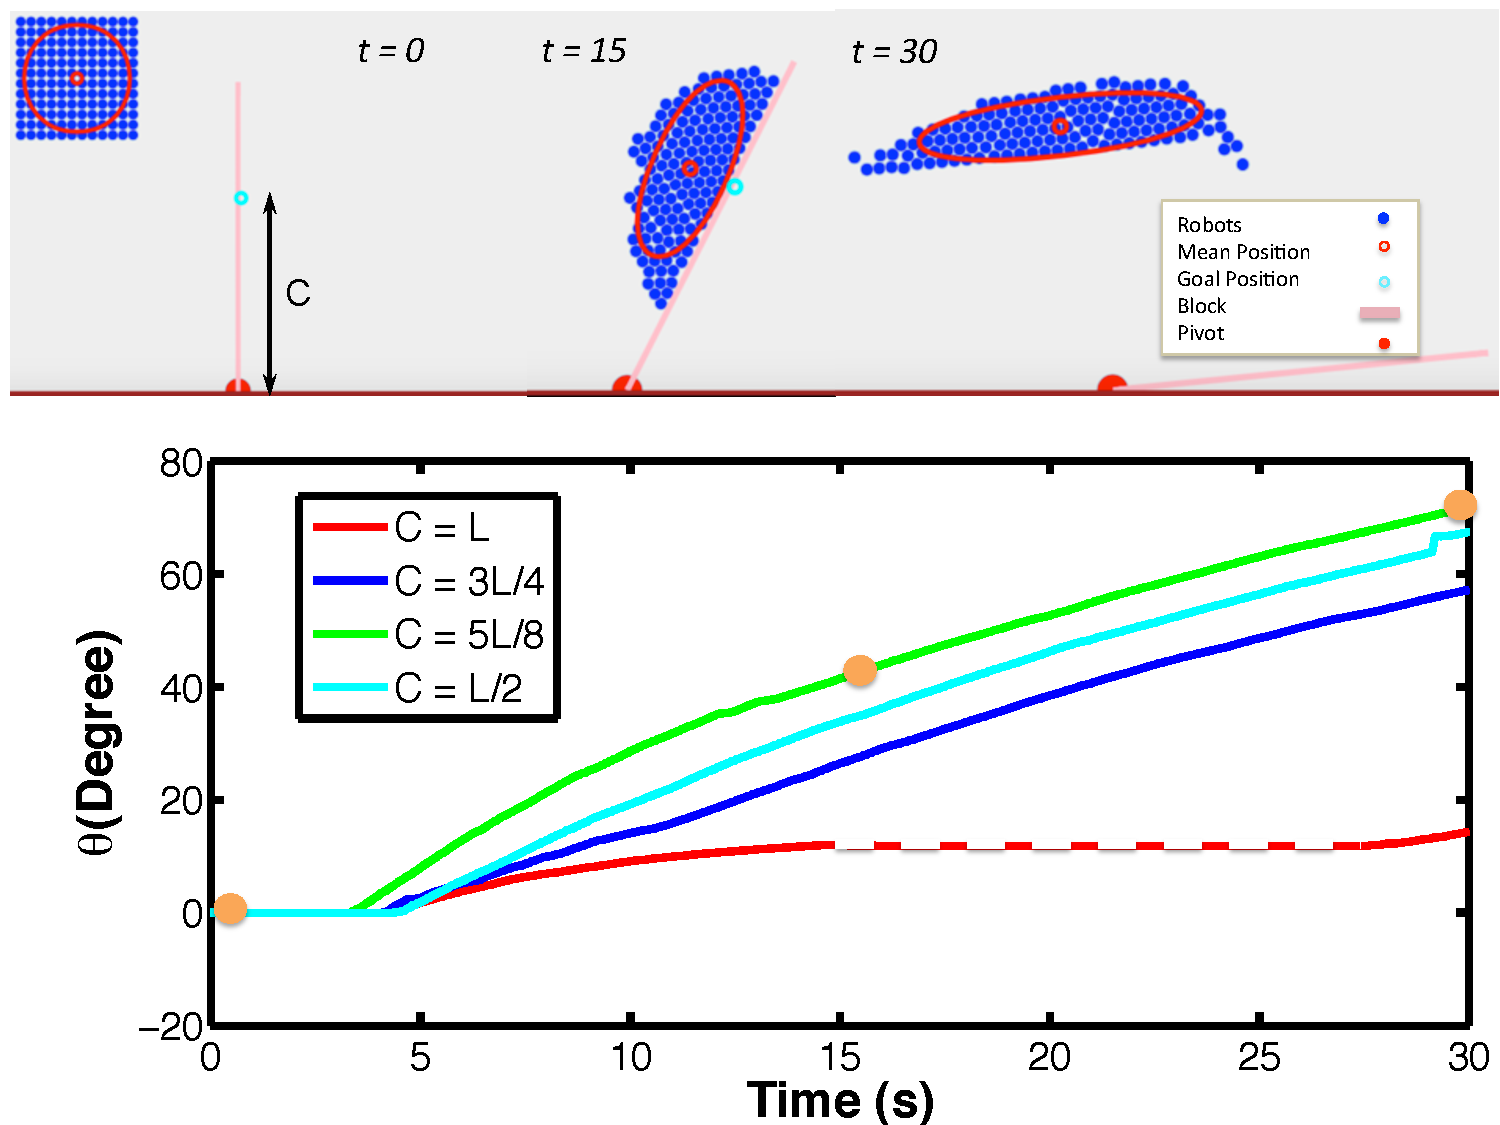
\includegraphics[width=0.8\columnwidth]{LFig.pdf}
\end{center}
\vspace{-1em}
\caption{\label{fig:LFig}
Simulation results from a swarm applying force to a hinged door. 
The swarm mean is steered toward a point $C$ units along the object from the pivot point. The red dashed line indicates the times that the swarm was in variance control mode.
% Simulation used 144 robots of diameter $0.2$ m with a standard deviation of less than $1.5$ m and an object length of $6$ m.
}
\vspace{-1em}
\end{figure}





\begin{figure}
\begin{center}
	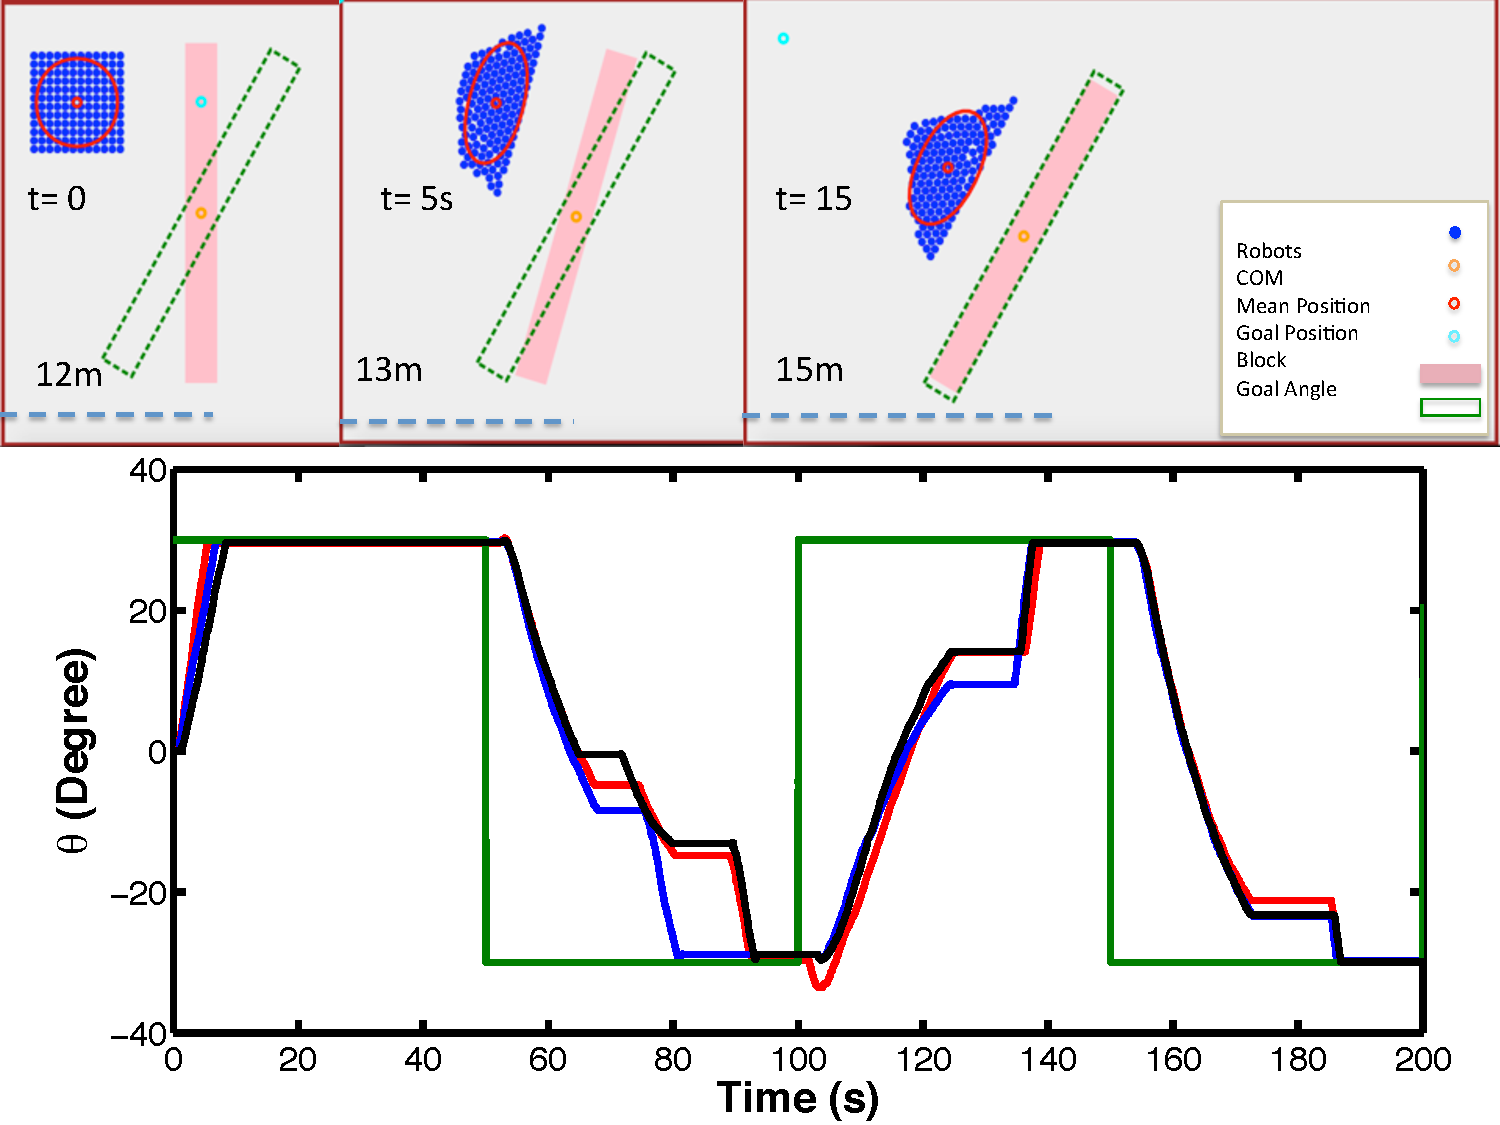
\includegraphics[width=0.8\columnwidth]{Orientation.pdf}
\end{center}
\vspace{-1em}
\caption{\label{fig:OrientCont}
Plot demonstrating  orientation control of a rectangular object. The green line is the goal orientation. Other lines show different random starting position of the swarm.% When the plot traces are constant the swarm is no longer pushing the object and instead is being regathered in a corner of the workspace until the variance is below a desired threshold. 
}
\vspace{-1em}
\end{figure}




